\documentclass[8pt]{article}
\usepackage{tikz}
\usepackage{graphicx} % for including images
\usetikzlibrary{automata, positioning}
\usepackage{amsmath}
\usepackage{hyperref}
\usepackage{float}

\usepackage{booktabs} % For better horizontal lines
\usepackage[table]{xcolor} % For row coloring (optional)

% Packages for fancy TOC
\usepackage{hyperref}  % Adds hyperlinks
\usepackage{tocloft}   % Customizes TOC
% Customize dot leaders in TOC
\renewcommand{\cftsecleader}{\cftdotfill{\cftdotsep}}
\begin{document}
\tableofcontents
\newpage
\section{DFA to accept strings of a’s and b’s that contain substring `aba`}

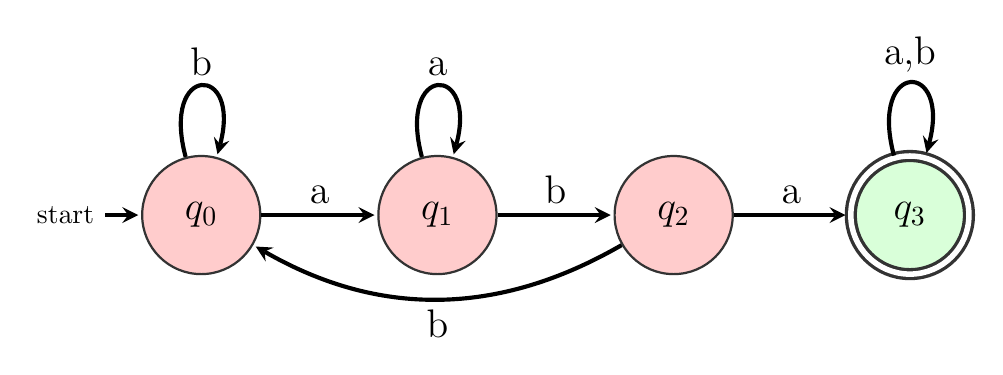
\begin{tikzpicture}[
    shorten >=1pt, 
    node distance=3cm, 
    on grid, 
    auto, 
    every state/.style={thick, minimum size=1.5cm, font=\Large, draw=black!80},
    every edge/.append style={line width=1.5pt, >=stealth, shorten >=1pt}
]

   % States with colors
   \node[state, initial, fill=red!20] (q0) {$q_0$};
   \node[state, fill=red!20] (q1) [right=of q0] {$q_1$};
   \node[state, fill=red!20] (q2) [right=of q1] {$q_2$};
   \node[state, accepting, fill=green!15, double distance=2pt, very thick] (q3) [right=of q2] {$q_3$};

   % Transitions
   \path[->]
   (q0) edge node {\Large a} (q1)
   (q0) edge [loop above] node {\Large b} ()

   (q1) edge [loop above] node {\Large a} ()
   (q1) edge node {\Large b} (q2)

   (q2) edge [bend left] node[below] {\Large b} (q0)
   (q2) edge node {\Large a} (q3)

   (q3) edge [loop above] node {\Large a,b} (); % loop for both 'a' and 'b'
\end{tikzpicture}


\section{To accept strings of a’s and b’s that start with baba}
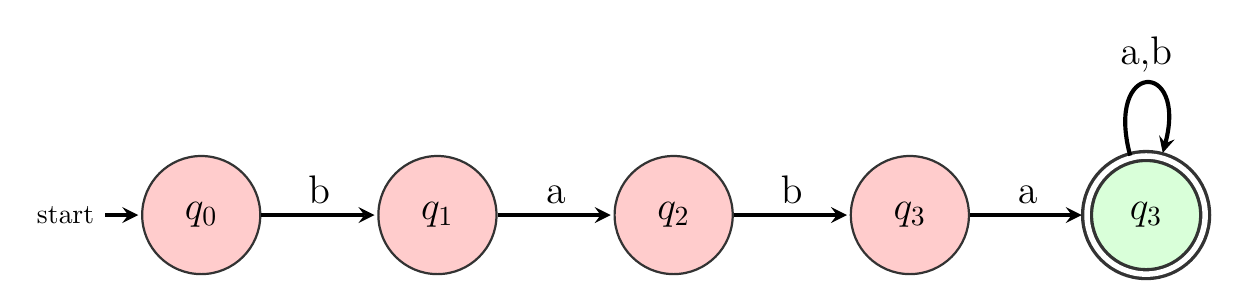
\begin{tikzpicture}[
    shorten >=1pt, 
    node distance=3cm, 
    on grid, 
    auto, 
    every state/.style={thick, minimum size=1.5cm, font=\Large, draw=black!80},
    every edge/.append style={line width=1.5pt, >=stealth, shorten >=1pt}
]

   % States with colors
   \node[state, initial, fill=red!20] (q0) {$q_0$};
   \node[state, fill=red!20] (q1) [right=of q0] {$q_1$};
   \node[state, fill=red!20] (q2) [right=of q1] {$q_2$};
   \node[state, fill=red!20] (q3) [right=of q2] {$q_3$};
   \node[state, accepting, fill=green!15, double distance=2pt, very thick] (q4) [right=of q3] {$q_3$};

   % Transitions
   \path[->]
   (q0) edge node {\Large b} (q1)
   (q1) edge node {\Large a} (q2)
   (q2) edge node {\Large b} (q3)

   (q3) edge node {\Large a} (q4)

   (q4) edge [loop above] node {\Large a,b} (); % loop for both 'a' and 'b' 
\end{tikzpicture}
\section{To accept strings of a’s and b’s that end with abba}
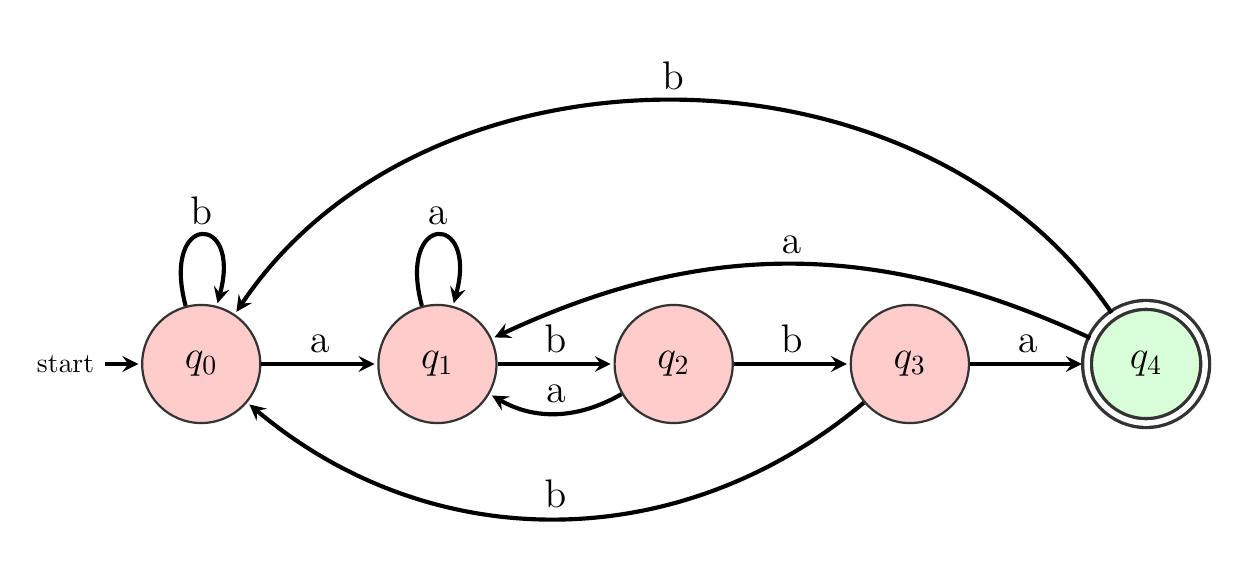
\begin{tikzpicture}[
    shorten >=1pt, 
    node distance=3cm, 
    on grid, 
    auto, 
    every state/.style={thick, minimum size=1.5cm, font=\Large, draw=black!80},
    every edge/.append style={line width=1.5pt, >=stealth, shorten >=1pt}
]

   % States with colors
   \node[state, initial, fill=red!20] (q0) {$q_0$};
   \node[state, fill=red!20] (q1) [right=of q0] {$q_1$};
   \node[state, fill=red!20] (q2) [right=of q1] {$q_2$};
   \node[state, fill=red!20] (q3) [right=of q2] {$q_3$};
   \node[state, accepting, fill=green!15, double distance=2pt, very thick] (q4) [right=of q3] {$q_4$};

   % Transitions
   \path[->]
   % (q0) edge node {\Large a} (q1)
   % (q0) edge [loop above] node {\Large b} ()

   % (q1) edge [loop above] node {\Large a} ()
   % (q1) edge node {\Large b} (q2)

   % (q2) edge [bend left] node[below] {\Large a} (q1)
   % (q2) edge node {\Large b} (q3)
   % (q3) edge [bend left] node[below] {\Large b} (q0)
   % (q3) edge node {\Large a} (q4)
   % (q4) edge [bend left] node {\Large a} (q1) 
   % (q4) edge [bend left] node {\Large b} (q0);

   (q0) edge node {\Large a} (q1)
   (q0) edge [loop above] node {\Large b} ()

   (q1) edge [loop above] node {\Large a} ()
   (q1) edge node {\Large b} (q2)

   (q2) edge [bend left] node[above] {\Large a} (q1)
   (q2) edge node {\Large b} (q3)

   (q3) edge [bend left=40] node[above] {\Large b} (q0) % bigger bend for clarity
   (q3) edge node {\Large a} (q4)

   (q4) edge[bend right=25] node[above] {\Large a} (q1)
   (q4) edge [bend right=56] node[above] {\Large b} (q0);

\end{tikzpicture}
\section{To accept strings of a’s and b’s that contains exactly two b’s}
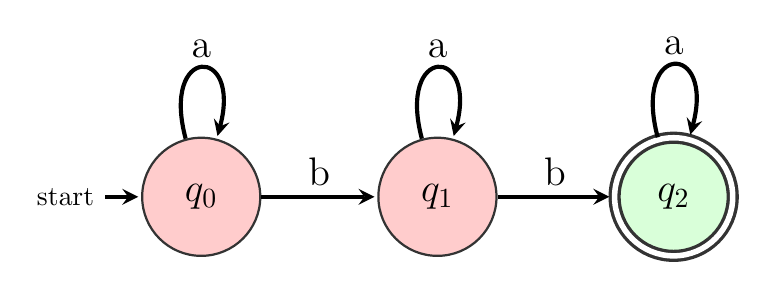
\begin{tikzpicture}[
    shorten >=1pt, 
    node distance=3cm, 
    on grid, 
    auto, 
    every state/.style={thick, minimum size=1.5cm, font=\Large, draw=black!80},
    every edge/.append style={line width=1.5pt, >=stealth, shorten >=1pt}
]

   % States with colors
   \node[state, initial, fill=red!20] (q0) {$q_0$};
   \node[state, fill=red!20] (q1) [right=of q0] {$q_1$};
   \node[state, accepting, fill=green!15, double distance=2pt, very thick] (q2) [right=of q1] {$q_2$};

   % Transitions
   \path[->]
   (q0) edge node {\Large b} (q1)
   (q0) edge [loop above] node {\Large a} ()

   (q1) edge [loop above] node {\Large a} ()
   (q1) edge node {\Large b} (q2)

 

   (q2) edge [loop above] node {\Large a} (); % loop for both 'a' and 'b'
\end{tikzpicture}
\section{}
% Insert an image at the top (adjust width as needed)
\begin{center}
    \includegraphics[width=1.3\textwidth]{slide_1_dfa/1.png} % replace logo.png with your file
\end{center}
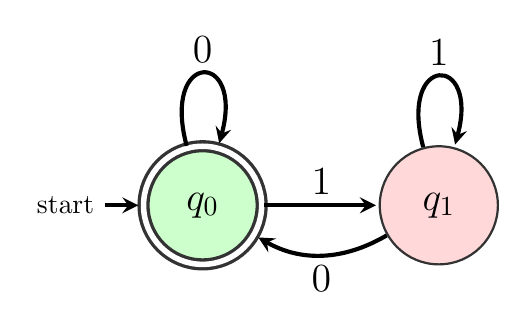
\begin{tikzpicture}[
    shorten >=1pt, 
    node distance=3cm, 
    on grid, 
    auto, 
    every state/.style={thick, minimum size=1.5cm, font=\Large, draw=black!80},
    every edge/.append style={line width=1.5pt, >=stealth, shorten >=1pt}
]

   % States with colors
   \node[state, initial, accepting, fill=green!20, double distance=2pt, very thick] (q0) {$q_0$};
   
   \node[state, fill=red!15] (q1) [right=of q0] {$q_1$};

   % Transitions
   \path[->]
   (q1) edge [bend left] node {\Large 0} (q0)
   (q0) edge node {\Large 1} (q1)
   (q1) edge [loop above] node {\Large 1} ()
   (q0) edge [loop above] node {\Large 0} ();

\end{tikzpicture}

\section{}
% Insert an image at the top (adjust width as needed)
\begin{center}
    \includegraphics[width=1.3\textwidth]{slide_1_dfa/2.png} % replace logo.png with your file
\end{center}
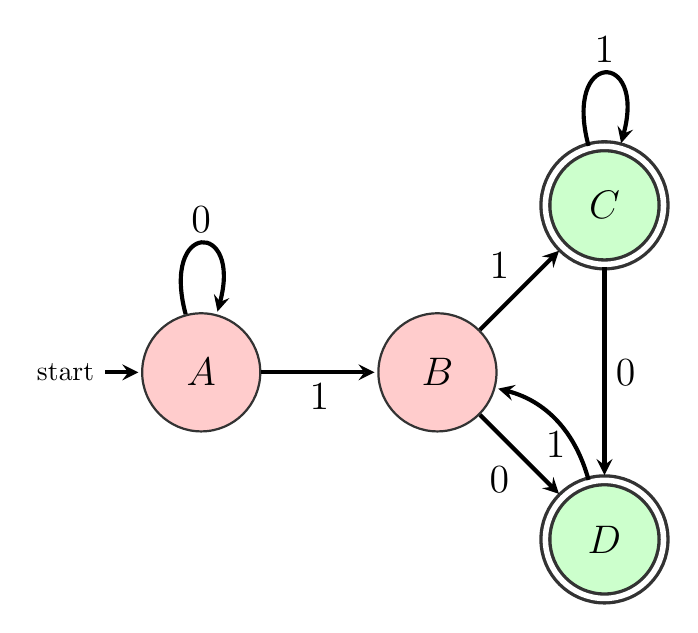
\begin{tikzpicture}[
    shorten >=1pt, 
    node distance=3cm, 
    on grid, 
    auto, 
    every state/.style={thick, minimum size=1.5cm, font=\Large, draw=black!80},
    every edge/.append style={line width=1.5pt, >=stealth, shorten >=1pt}
]

   % States
   \node[state, initial, fill=red!20] (A) {$A$};
   \node[state, fill=red!20] (B) [right=of A] {$B$};
   \node[state, accepting, fill=green!20, double distance=2pt, very thick] (C) [above right=of B] {$C$};
   \node[state, accepting, fill=green!20, double distance=2pt, very thick] (D) [below right=of B] {$D$};

   % Transitions
   \path[->]
   (A) edge [loop above] node {\Large 0} ()
   (A) edge node[below] {\Large 1} (B)
   (B) edge node[above left] {\Large 1} (C)
   (B) edge node[below left] {\Large 0} (D)
   (C) edge [loop above] node {\Large 1} ()
   (C) edge node[right] {\Large 0} (D)
   (D) edge [bend right=30] node[below] {\Large 1} (B);

\end{tikzpicture}

\section{}
% Insert an image at the top (adjust width as needed)
\begin{center}
    \includegraphics[width=1.3\textwidth]{slide_1_dfa/3.png} % replace logo.png with your file
\end{center}
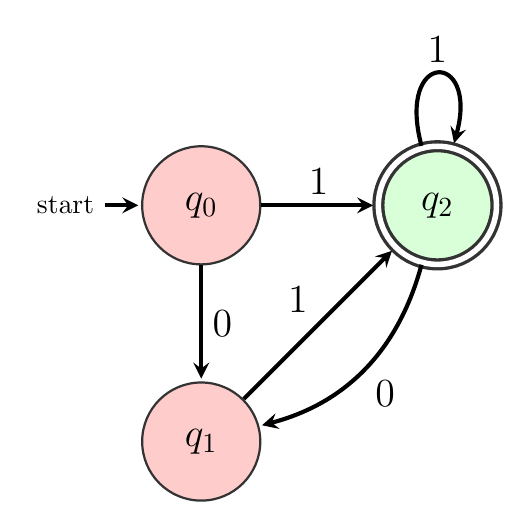
\begin{tikzpicture}[
    shorten >=1pt, 
    node distance=3cm, 
    on grid, 
    auto, 
    every state/.style={thick, minimum size=1.5cm, font=\Large, draw=black!80},
    every edge/.append style={line width=1.5pt, >=stealth, shorten >=1pt}
]

   % States with colors
   \node[state, initial, fill=red!20] (q0) {$q_0$};
   \node[state, fill=red!20] (q1) [below =of q0] {$q_1$};
   \node[state, accepting, fill=green!15, double distance=2pt, very thick] (q2) [right=of q0] {$q_2$};

   % Transitions
   \path[->]
   (q0) edge node {\Large 1} (q2)
   (q0) edge node {\Large 0} (q1)
   (q1) edge node {\Large 1} (q2)
   (q2) edge [bend left] node {\Large 0} (q1)
   (q2) edge [loop above] node {\Large 1} (); % loop for both 'a' and 'b'
\end{tikzpicture}
\section{With 5 nfa state, construct a dfa whcih lead to worst case state scenario. Final output will show 32 state}

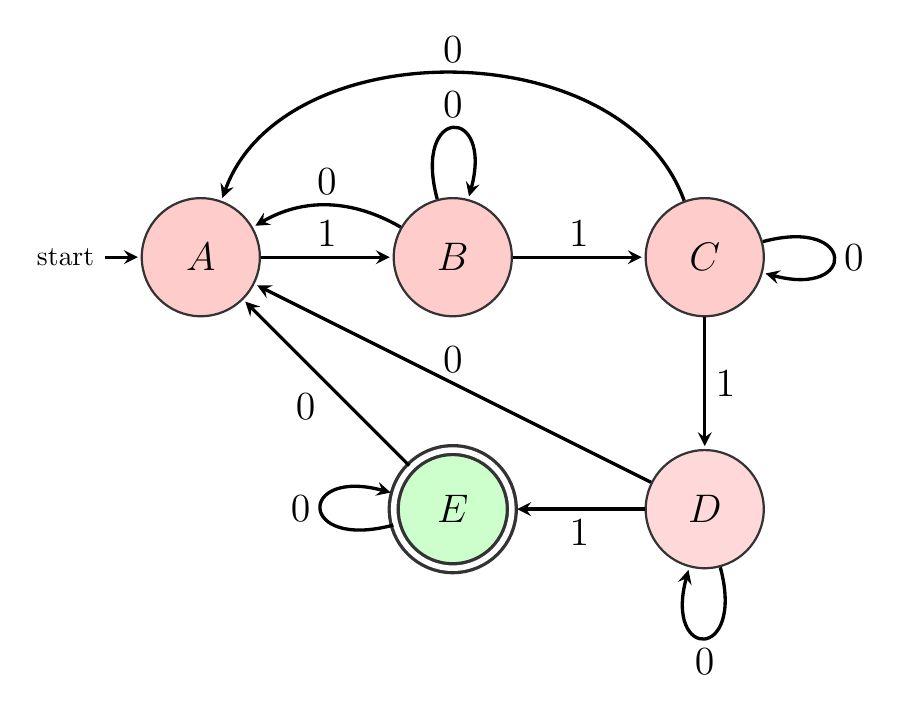
\begin{tikzpicture}[
    shorten >=1pt, 
    node distance=3.2cm, 
    on grid, 
    auto, 
    every state/.style={thick, minimum size=1.5cm, font=\Large, draw=black!80},
    every edge/.append style={line width=1.2pt, >=stealth, shorten >=1pt}
]

   % States
   \node[state, initial, fill=red!20] (A) {$A$}; % initial
   \node[state, fill=red!20] (B) [right=of A] {$B$};
   \node[state, fill=red!20] (C) [right=of B] {$C$};
   \node[state, fill=red!15] (D) [below=of C] {$D$};
   \node[state, accepting, fill=green!20, double distance=2pt, very thick] (E) [left=of D] {$E$};

   % Transitions (mod 5 machine)
   \path[->]
   (A) edge node {\Large 1} (B)

   (B) edge[loop above] node {\Large 0} ()
       edge node  {\Large 1} (C)
       edge [bend right] node [above] {\Large 0} (A)

   (C) edge node {\Large 1} (D)
        edge [loop right] node {\Large 0} ()
        edge [bend right = 70]  node [above] {\Large 0} (A)

   (D) edge node[above] {\Large 0} (A)
        edge node [below] {\Large 1} (E)
        edge [loop below] node  {\Large 0} ()

   (E) edge [loop left] node {\Large 0} ()
        edge node {\Large 0} (A);

\end{tikzpicture}
\subsubsection{Transition Table of the DFA}
\begin{table}[H]
    \centering
    \renewcommand{\arraystretch}{1.3} % Increase row height for readability
    \begin{tabular}{|c|c|c|}
        \hline
        \rowcolor{gray!20} % Optional: header background color
        \textbf{DFA State} & \textbf{On 0} & \textbf{On 1} \\
        \hline
        \{A\} & $\emptyset$
 & \{ B\} \\
        \hline
        $\emptyset$ & $\emptyset$
 & $\emptyset$ \\
        \hline
        \{B\} & \{A, B\} & \{ C\} \\
        \hline
        \{ C\} & \{A, C\} & \{ D\} \\
        \hline
        \{A, B\} & \{A, B\} & \{B, C\} \\
        \hline
        \{A, C\} & \{A, C\} & \{B, D\} \\
        \hline
        \{D\} & \{A, D\} & \{E\} \\
        \hline
        \{B, C\} & \{A, B, C\} & \{C, D\} \\
        \hline
        \{B, D\} & \{A, B, D\} & \{C, E\} \\
        \hline
        \{A, D\} & \{A, D\} & \{B, E\} \\
        \hline
        \{ E\} & \{A, E\} & \{\} \\
        \hline
        \{C, D\} & \{A, C, D\} & \{D, E\} \\
        \hline
        \{A, B, C\} & \{A, B, C\} & \{B, C, D\} \\
        \hline
        \{B, E\} & \{A, B, E\} & \{C\} \\
        \hline
        \{A, C, D\} & \{A, C, D\} & \{B, D, E\} \\
        \hline
        \{D, E\} & \{A, D, E\} & \{E\} \\
        \hline
        \{B, C, D\} & \{A, B, C, D\} & \{C, D, E\} \\
        \hline
        \{C, D, E\} & \{A, C,D, E\} & \{D, E\} \\
        \hline
        \{A, B, C, D\} & \{A, B, C, D\} & \{B, C, D, E\} \\
        \hline
        \{B, C, D, E\} & \{A, B, C, D, E\} & \{C, D, E\} \\
        \hline
        \{A, E\} & \{A, E\} & \{B\} \\
        \hline
        \{A, D, E\} & \{A, D, E\} & \{B, E\} \\
        \hline
        \{A, C, D, E\} & \{A, C, D, E\} & \{B, C, D\} \\
        \hline
        \{A,B,C, D, E\} & \{A, B, C, D, E\} & \{B,C,D, E\} \\
        \hline
        \{A, B, D\} & \{A, B, D\} & \{B, C, E\} \\
        \hline
        \{C, E\} & \{A, C, E\} & \{D\} \\
        \hline
        \{B, C, E\} & \{A, B, C, E\} & \{C, D\} \\
        \hline
        \{A, C, E\} & \{A, C, E\} & \{B, D\} \\
        \hline
        \{A, B, C, E\} & \{A, B, C, E\} & \{B, C, D\} \\
        \hline
        \{A, B, E\} & \{A, B, E\} & \{B, C\} \\
        \hline
        \{B, D, E\} & \{A, B, D, E\} & \{C, E\} \\
        \hline
        \{A, B, D, E\} & \{A, B, D, E\} & \{B, C, E\} \\
        \hline
        
    \end{tabular}
    \caption{DFA Transition Table}
    \label{tab:dfa_transition}
\end{table}



\section{Construct DFA, which accepts set of all strings over {0, 1} which interpreted as binary number is divisible by 3. }
\begin{center}
    \includegraphics[width=1.3\textwidth]{divisible/3.png} 
\end{center}
\section{Construct DFA, which accepts set of all strings over {0, 1} which interpreted as binary number is divisible by 4. }
\begin{center}
    \includegraphics[width=1.3\textwidth]{divisible/4.png} % replace logo.png with your file
\end{center}
\section{ DFA that checks if a string ends with "01" or "10"}
\begin{center}
    \includegraphics[width=1.3\textwidth]{ending/10_01.png} % replace logo.png with your file
\end{center}
\section{DFA to accept Binary strings that starts or ends with "01"}
\begin{center}
    \includegraphics[width=1.3\textwidth]{ending/end_start.png} % replace logo.png with your file
\end{center}
\section{DFA of a string with at least two 0’s and at least two 1’s}
\begin{center}
    \includegraphics[width=1.3\textwidth]{pictures/12.png} % replace logo.png with your file
\end{center}
\subsection{RE}
\[
\begin{aligned}
&(0+1)^{*}0(0+1)^{*}0(0+1)^{*}1(0+1)^{*}1(0+1)^{*} \\
&\qquad+\; (0+1)^{*}0(0+1)^{*}1(0+1)^{*}0(0+1)^{*}1(0+1)^{*} \\
&\qquad+\; (0+1)^{*}0(0+1)^{*}1(0+1)^{*}1(0+1)^{*}0(0+1)^{*} \\
&\qquad+\; (0+1)^{*}1(0+1)^{*}0(0+1)^{*}0(0+1)^{*}1(0+1)^{*} \\
&\qquad+\; (0+1)^{*}1(0+1)^{*}0(0+1)^{*}1(0+1)^{*}0(0+1)^{*} \\
&\qquad+\; (0+1)^{*}1(0+1)^{*}1(0+1)^{*}0(0+1)^{*}0(0+1)^{*}
\end{aligned}
\]


\section{ accept 00 and 11 at the end of a string}
\begin{center}
    \includegraphics[width=1.3\textwidth]{pictures/13.png} % replace logo.png with your file
\end{center}
\section{DFA for accepting the language $L = \{ a^n b^m \mid n+m \text{ is even} \}$}
\begin{center}
    \includegraphics[width=1.3\textwidth]{pictures/13.png} % replace logo.png with your file
\end{center}
\section{DFA of a string in which 2nd symbol from RHS is 'a'}
\begin{center}
    \includegraphics[width=1.3\textwidth]{pictures/15.png} % replace logo.png with your file
\end{center}
\begin{center}
    \includegraphics[width=1.3\textwidth]{pictures/15_nfa.png} % replace logo.png with your file
\end{center}
\section{Draw a deterministic and non-deterministic finite automate which either starts with 01 or end with 01 of a string containing 0, 1 in it, e.g., 01010100 but not 000111010. }
\begin{center}
    \includegraphics[width=1.3\textwidth]{pictures/16_nfa.png} % replace logo.png with your file
\end{center}
\begin{center}
    \includegraphics[width=1.3\textwidth]{pictures/16.png} % replace logo.png with your file
\end{center}
\section{ Draw a non-deterministic finite automate which starts with 01 and ends with 01 of a string containing 0, 1 in it, e.g., 01000101 but not 000111001.}
\begin{center}
    \includegraphics[width=1.3\textwidth]{pictures/17.png} % replace logo.png with your file
\end{center}
\section{Construct a DFA that Start With aa or bb}
\begin{center}
    \includegraphics[width=1.3\textwidth]{pictures/18.png} % replace logo.png with your file
\end{center}
\section{DFA that Accepts All the Strings With At Least 1 'a' and Exactly 2 b's}
\begin{center}
    \includegraphics[width=1.3\textwidth]{pictures/19.png} % replace logo.png with your file
\end{center}
\section{Program to build a DFA to accept strings that start and end with same character}
\begin{center}
    \includegraphics[width=1.3\textwidth]{pictures/20.png} % replace logo.png with your file
\end{center}
\section{at most two b}
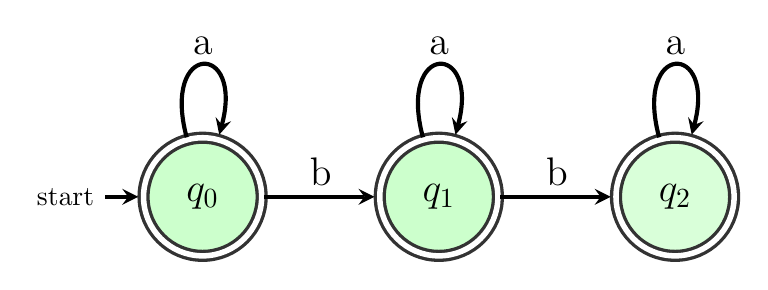
\begin{tikzpicture}[
    shorten >=1pt, 
    node distance=3cm, 
    on grid, 
    auto, 
    every state/.style={thick, minimum size=1.5cm, font=\Large, draw=black!80},
    every edge/.append style={line width=1.5pt, >=stealth, shorten >=1pt}
]

   % States with colors
   \node[state, accepting, initial, fill=green!20, double distance=2pt, very thick] (q0) {$q_0$};
   \node[state, accepting, fill=green!20, double distance=2pt, very thick] (q1) [right=of q0] {$q_1$};
   \node[state, accepting, fill=green!15, double distance=2pt, very thick] (q2) [right=of q1] {$q_2$};

   % Transitions
   \path[->]
   (q0) edge node {\Large b} (q1)
   (q0) edge [loop above] node {\Large a} ()

   (q1) edge [loop above] node {\Large a} ()
   (q1) edge node {\Large b} (q2)

 

   (q2) edge [loop above] node {\Large a} (); % loop for both 'a' and 'b'
\end{tikzpicture}
\subsection{RE}
\[
\Huge \mathbf{
a^{*} \;+\; a^{*} b a^{*} \;+\; a^{*} b a^{*} b a^{*}
}
\]



\section{at least 2 b}
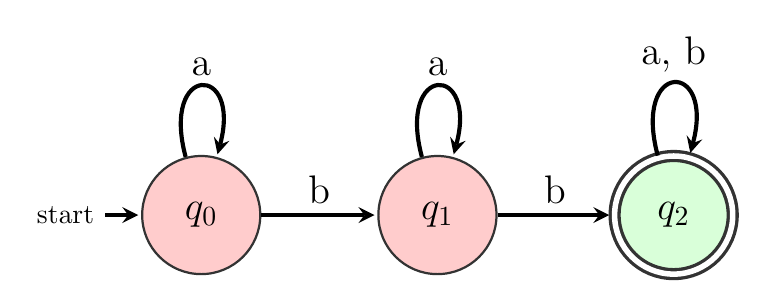
\begin{tikzpicture}[
    shorten >=1pt, 
    node distance=3cm, 
    on grid, 
    auto, 
    every state/.style={thick, minimum size=1.5cm, font=\Large, draw=black!80},
    every edge/.append style={line width=1.5pt, >=stealth, shorten >=1pt}
]

   % States with colors
   \node[state, initial, fill=red!20] (q0) {$q_0$};
   \node[state, fill=red!20] (q1) [right=of q0] {$q_1$};
   \node[state, accepting, fill=green!15, double distance=2pt, very thick] (q2) [right=of q1] {$q_2$};

   % Transitions
   \path[->]
   (q0) edge node {\Large b} (q1)
   (q0) edge [loop above] node {\Large a} ()

   (q1) edge [loop above] node {\Large a} ()
   (q1) edge node {\Large b} (q2)
   
   (q2) edge [loop above] node {\Large a, b} (); % loop for both 'a' and 'b'
\end{tikzpicture}
\[
\Huge \mathbf{
a^{*} b a^{*} b (a+b)^{*}
}
\]

\section{DFA accepting odd number of 0s and odd number of 1s}
\begin{center}
    \includegraphics[width=1.3\textwidth]{pictures/23.png} % replace logo.png with your file
\end{center}
\section{Incourse - 27}
\subsection{ DFA and Regular Expression over the Alphabet $\{0,1,2\}$}

\large{
A Deterministic Finite Automaton (DFA) and regular expression are to be constructed over the
alphabet $\{0,1,2\}$ to accept only those strings that satisfy the following constraints:

\begin{itemize}
    \item If the string starts with $1$, it must contain at least one occurrence of $0$ 
          (there is no restriction on the number of $1$s or $2$s in the string).
    \item If the string starts with $2$, it must contain exactly one occurrence of $2$, 
          and the second-to-last symbol of the string must always be $0$.
\end{itemize}
}

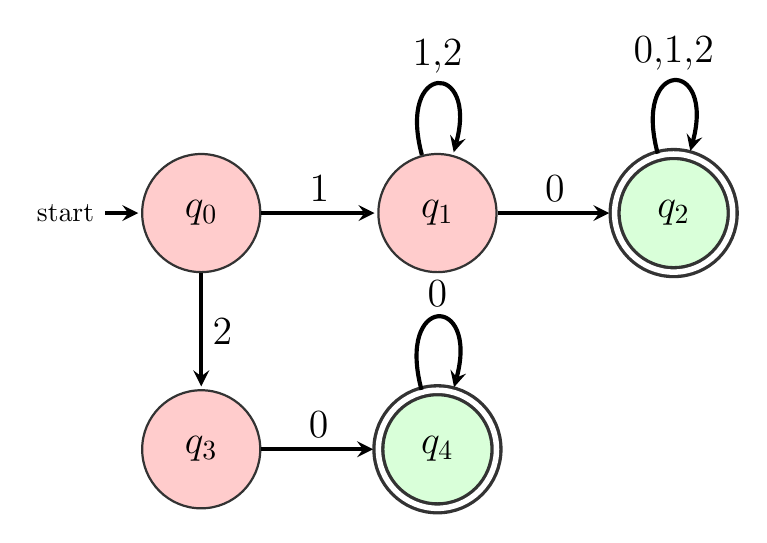
\begin{tikzpicture}[
    shorten >=1pt, 
    node distance=3cm, 
    on grid, 
    auto, 
    every state/.style={thick, minimum size=1.5cm, font=\Large, draw=black!80},
    every edge/.append style={line width=1.5pt, >=stealth, shorten >=1pt}
]

   % States
   \node[state, initial, fill=red!20] (q0) {$q_0$}; % Start
   \node[state, fill=red!20] (q1) [right=of q0] {$q_1$}; % seen 1, no 0 yet
   \node[state, accepting, fill=green!15, double distance=2pt, very thick] (q2) [right=of q1] {$q_2$}; % seen 1, at least one 0
   \node[state, fill=red!20] (q3) [below=of q0] {$q_3$}; % seen 2, second-to-last 0 not satisfied
   \node[state, accepting, fill=green!15, double distance=2pt, very thick] (q4) [right=of q3] {$q_4$}; % seen 2, second-to-last 0 satisfied

   % Transitions for strings starting with 1
   \path[->]
   (q0) edge node {\Large 1} (q1)
   (q0) edge node {\Large 2} (q3)
   (q1) edge node {\Large 0} (q2)
   (q1) edge [loop above] node {\Large 1,2} ()
   (q2) edge [loop above] node {\Large 0,1,2} ();

   % Transitions for strings starting with 2
   \path[->]
   % (q4) edge [bend left] node {\Large 2} (q3)
   (q3) edge node {\Large 0} (q4)
   % (q3) edge [loop left] node {\Large 1} ()
   (q4) edge [loop above] node {\Large 0} (); % 0, 1
\end{tikzpicture}
\subsection{DFA for recognizing relational operators}
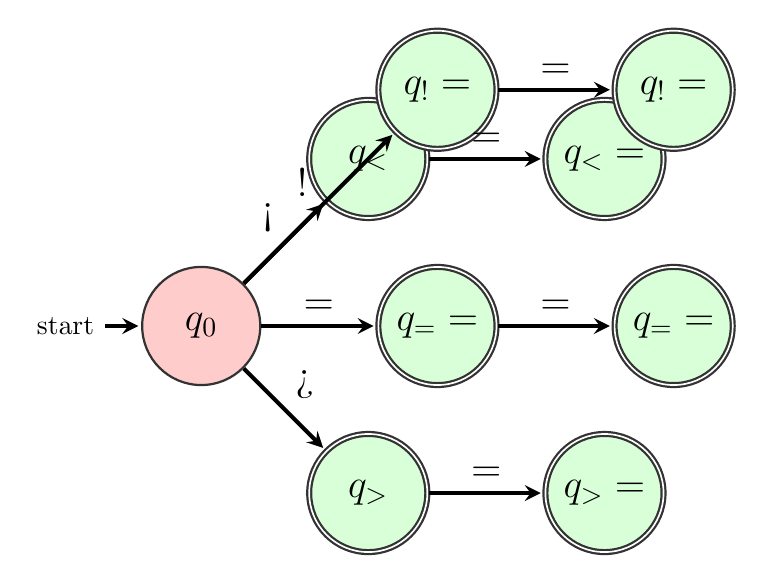
\begin{tikzpicture}[
    shorten >=1pt, 
    node distance=3cm, 
    on grid, 
    auto, 
    every state/.style={thick, minimum size=1.5cm, font=\Large, draw=black!80},
    every edge/.append style={line width=1.5pt, >=stealth, shorten >=1pt}
]

    % States
    \node[state, initial, fill=red!20] (q0) {$q_0$};
    \node[state, accepting, fill=green!15] (q1) [above right=of q0] {$q_<$};
    \node[state, accepting, fill=green!15] (q2) [below right=of q0] {$q_>$};
    \node[state, accepting, fill=green!15] (q3) [right=of q0] {$q_==$};
    \node[state, accepting, fill=green!15] (q4) [above=of q3] {$q_!=$};
    \node[state, accepting, fill=green!15] (q_le) [right=of q1] {$q_<= $};
    \node[state, accepting, fill=green!15] (q_ge) [right=of q2] {$q_>= $};
    \node[state, accepting, fill=green!15] (q_eq) [right=of q3] {$q_== $};
    \node[state, accepting, fill=green!15] (q_ne) [right=of q4] {$q_!= $};

    % Transitions
    \path[->]
    (q0) edge node {\Large <} (q1)
    (q0) edge node {\Large >} (q2)
    (q0) edge node {\Large =} (q3)
    (q0) edge node {\Large !} (q4)

    (q1) edge node {\Large =} (q_le)
    (q2) edge node {\Large =} (q_ge)
    (q3) edge node {\Large =} (q_eq)
    (q4) edge node {\Large =} (q_ne);
\end{tikzpicture}
\subsection{Convert the given NFA with \(\varepsilon\)-transitions into an equivalent Deterministic Finite Automaton (DFA). What would be the worst-case outcome of such a transformation in terms of the number of nodes?}

\begin{center}
    \includegraphics[width=1.3\textwidth]{27_incourse/2.png} % replace logo.png with your file
\end{center}
\subsubsection{Transition Table of the DFA}


\begin{table}[h!]
    \centering
    \renewcommand{\arraystretch}{1.3} % Increase row height for readability
    \begin{tabular}{|c|c|c|}
        \hline
        \rowcolor{gray!20} % Optional: header background color
        \textbf{DFA State} & \textbf{On 0} & \textbf{On 1} \\
        \hline
        \{A\} & \{A,B\} & \{C\} \\
        \hline
        \{A,B\} & \{A,B\} & \{C\} \\
        \hline
        \{C\} & \{A,B\} & \{A,B,D\} \\
        \hline
        \{A,B,D\} & \{A,B,C\} & \{C\} \\
        \hline
        \{A,B,C\} & \{A,B\} & \{A,B,C,D\} \\
        \hline
        \{A,B,C,D\} & \{A,B,C\} & \{A,B,C,D\} \\
        \hline
    \end{tabular}
    \caption{DFA Transition Table}
    \label{tab:dfa_transition}
\end{table}

Start state: $\{A\}$ \\
Accepting states: $\{A,B,D\}, \{A,B,C,D\}$

\subsubsection{DFA Diagram}

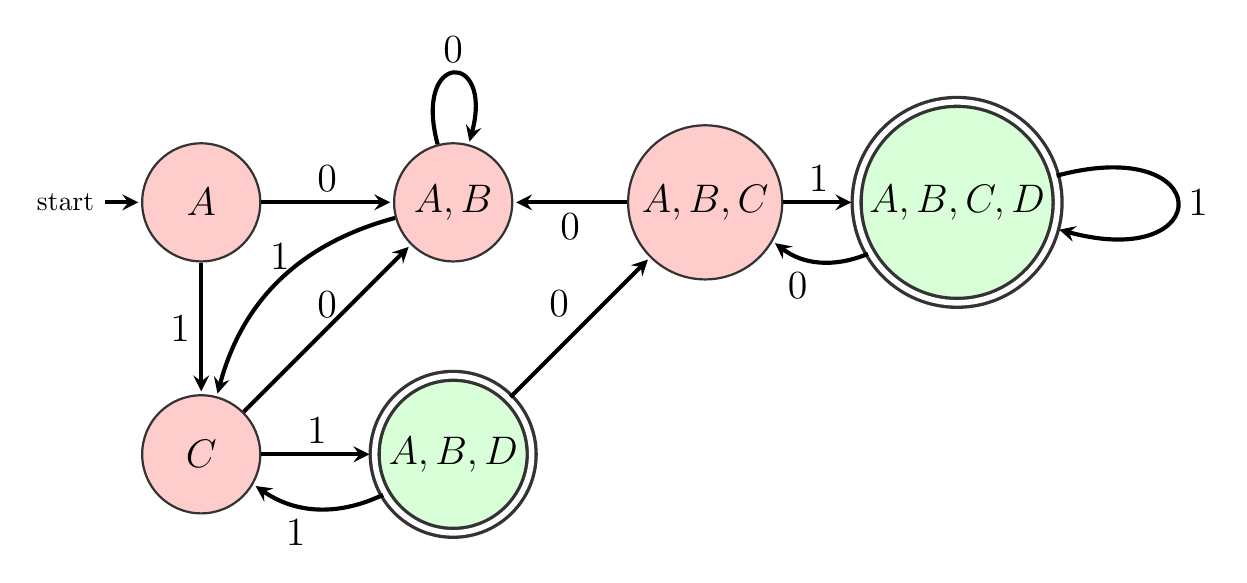
\begin{tikzpicture}[
    shorten >=1pt, 
    node distance=3.2cm, 
    on grid, 
    auto, 
    every state/.style={thick, minimum size=1.5cm, font=\Large, draw=black!80},
    every edge/.append style={line width=1.5pt, >=stealth, shorten >=1pt}
]

   % States
   \node[state, initial, fill=red!20] (q0) {$A$};
   \node[state, fill=red!20] (q1) [right=of q0] {$A,B$};
   \node[state, fill=red!20] (q2) [below=of q0] {$C$};
   \node[state, accepting, fill=green!15, double distance=2pt, very thick] (q3) [right=of q2] {$A,B,D$};
   \node[state, fill=red!20] (q4) [right=of q1] {$A,B,C$};
   \node[state, accepting, fill=green!15, double distance=2pt, very thick] (q5) [right=of q4] {$A,B,C,D$};

   % Transitions
   \path[->]
   (q0) edge node {\Large 0} (q1)
   (q0) edge node[left] {\Large 1} (q2)
   (q1) edge [loop above] node {\Large 0} ()
   (q1) edge [bend right] node [above] {\Large 1} (q2)
   (q2) edge node[above] {\Large 0} (q1)
   (q2) edge node {\Large 1} (q3)
   (q3) edge node {\Large 0} (q4)
   (q3) edge[bend left] node {\Large 1} (q2)
   (q4) edge node {\Large 0} (q1)
   (q4) edge node {\Large 1} (q5)
   (q5) edge[loop right] node {\Large 1} ()
   (q5) edge[bend left] node {\Large 0} (q4);
\end{tikzpicture}

\subsubsection{Worst-case Outcome}
For an NFA with $n$ states, the subset-construction may produce a DFA with up to $2^n$ states.  
Here $n=4$, so the worst-case DFA has $2^4 = 16$ states.  
In this particular case, only 6 DFA states are reachable.
\subsection{Final 27 (1b)}

\begin{center}
    \includegraphics[width=1.3\textwidth]{27_incourse/final_1b.png} % replace logo.png with your file
\end{center}
\subsubsection{Transition Table of the DFA}

\begin{table}[H]
    \centering
    \renewcommand{\arraystretch}{1.3} % Increase row height for readability
    \begin{tabular}{|c|c|c|}
        \hline
        \rowcolor{gray!20} % Optional: header background color
        \textbf{DFA State} & \textbf{On 0} & \textbf{On 1} \\
        \hline
        \{S, A\} & \{A,C, D, E\} & \{A, B, C\} \\
        \hline
        \{A,C, D, E\} & \{D, E\} & \{A, B, C\} \\
        \hline
        \{A, B, C\} & \{D, E\} & \{B, E, D\} \\
        \hline
        \{D, E\} & \{\} & \{C, A\} \\
        \hline
        \{B, D, E\} & \{D\} & \{A,C,D, E\} \\
        \hline
        \{C, A\} & \{D, E\} & \{B\} \\
        \hline
        \{D\} & \{\} & \{C, A\} \\
        \hline
        \{B\} & \{D\} & \{D, E\} \\
        \hline
    \end{tabular}
    \caption{DFA Transition Table}
    \label{tab:dfa_transition}
\end{table}

Start state: $\{S, A\}$ \\
Accepting states: $\{A,C,D, E\}, \{D, E\}, \{B, E, D\}$

\subsection{DFA}
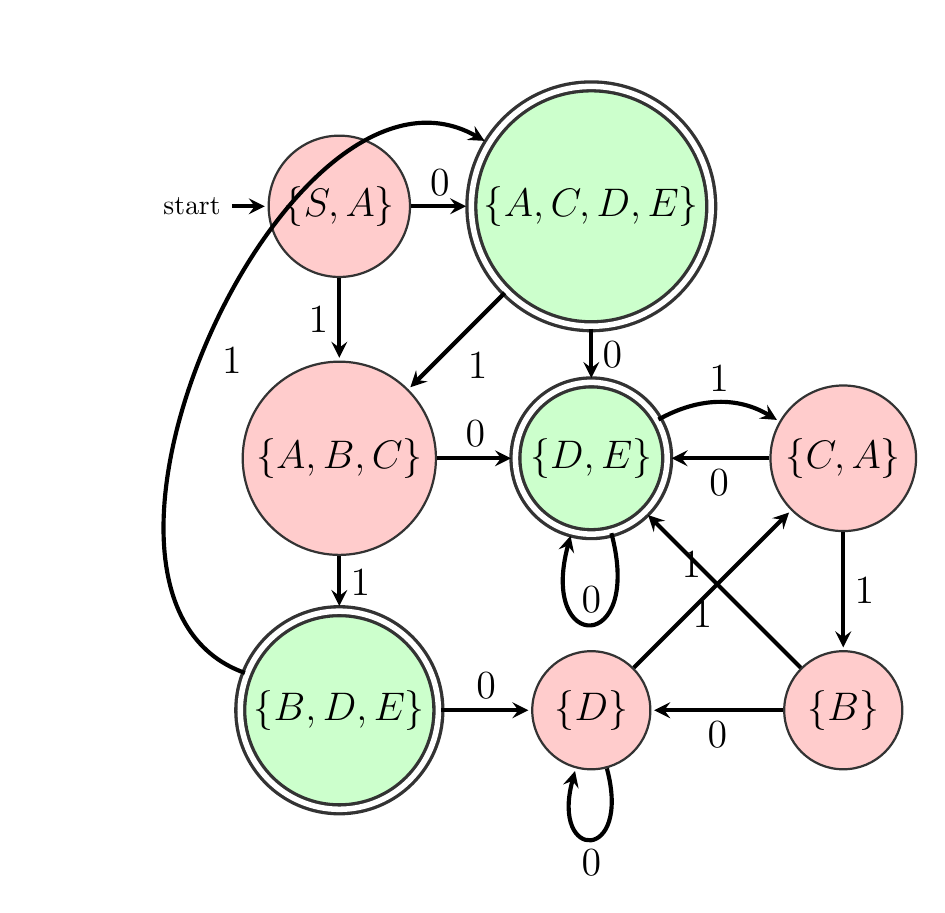
\begin{tikzpicture}[
    shorten >=1pt, 
    node distance=3.2cm, 
    on grid, 
    auto, 
    every state/.style={thick, minimum size=1.5cm, font=\Large, draw=black!80},
    every edge/.append style={line width=1.5pt, >=stealth, shorten >=1pt}
]

   % States
   \node[state, initial, fill=red!20] (q0) {$\{S,A\}$};
   \node[state, accepting, fill=green!20, double distance=2pt, very thick] (q1) [right=of q0] {$\{A,C,D,E\}$};
   \node[state, fill=red!20] (q2) [below=of q0] {$\{A,B,C\}$};
   \node[state, fill=green!20, double distance=2pt, very thick] (q3) [right=of q2] {$\{D,E\}$};
   \node[state,accepting, fill=green!20, double distance=2pt, very thick] (q4) [below=of q2] {$\{B,D,E\}$};
   \node[state, fill=red!20] (q5) [right=of q3] {$\{C,A\}$};
   \node[state, fill=red!20] (q6) [below=of q3] {$\{D\}$};
   \node[state, fill=red!20] (q7) [right=of q6] {$\{B\}$};

   % Transitions
   \path[->]
   (q0) edge node {\Large 0} (q1)
   (q0) edge node[left] {\Large 1} (q2)
   
   (q1) edge node {\Large 0} (q3)
   (q1) edge node {\Large 1} (q2)
   
   (q2) edge node {\Large 0} (q3)
   (q2) edge node {\Large 1} (q4)
   
   (q3) edge [loop below] node [above] {\Large 0} ()
   (q3) edge [bend left] node {\Large 1} (q5)
   
   (q4) edge node {\Large 0} (q6)
   (q4) edge [bend left = 95] node [below right] {\Large 1} (q1)
   
   (q5) edge node {\Large 0} (q3)
   (q5) edge node {\Large 1} (q7)
   
   (q6) edge [loop below] node {\Large 0} ()
   (q6) edge node {\Large 1} (q5)
   
   (q7) edge node {\Large 0} (q6)
   (q7) edge node {\Large 1} (q3);
\end{tikzpicture}
\subsection{Final 2 a}
\begin{center}
    \includegraphics[width=1.3\textwidth]{27_incourse/2a_final.png} % replace logo.png with your file
\end{center}

% \[
% \begin{array}{|c|c|c|c|c|}
% \hline
% \text{Present State} & \text{Next state for } \# & \text{Next state for } @ & \text{Next state for } \% & \text{Output } \lambda \\
% \hline
% \to A & B & A & E & \$ \\
% B & B & C & D & \pounds \\
% C & E & E & C & \$ \\
% D & A & D & C & \& \\
% E & D & B & A & * \\
% \hline
% \end{array}
% \]

% \subsection*{Equivalent Mealy Machine}

% In Mealy machine, the output is assigned to the transition:
% \[
% \lambda'(q, x) = \lambda(\delta(q, x)).
% \]

% \[
% \begin{array}{|c|c|c|c|}
% \hline
% \text{Present State} & \text{Input } \# & \text{Input } @ & \text{Input } \% \\
% \hline
% A & B,\pounds & A,\$ & E,* \\
% \hline
% B & B,\pounds & C,\$ & D,\& \\
% \hline
% C & E,* & E,* & C,\$ \\
% \hline
% D & A,\$ & D,\& & C,\$ \\
% \hline
% E & D,\& & B,\pounds & A,\$ \\

% \hline
% \end{array}
% \]
\bigskip

\noindent
\begin{tabular}{|c||>{\centering}p{1.8cm}|>{\centering}p{1.6cm}
                |>{\centering}p{1.8cm}|>{\centering}p{1.6cm}
                |>{\centering}p{1.8cm}|>{\centering\arraybackslash}p{1.6cm}|}
\hline
\textbf{Present} & \multicolumn{2}{c|}{\textbf{Input: \#}} 
                & \multicolumn{2}{c|}{\textbf{Input: @}} 
                & \multicolumn{2}{c|}{\textbf{Input: \%}} \\
\cline{2-7}
\textbf{State} & \textbf{State} & \textbf{Output} 
               & \textbf{State} & \textbf{Output}
               & \textbf{State} & \textbf{Output} \\
\hline\hline
$\to A$ & B & \pounds & A & \$ & E & * \\
\hline
B      & B & \pounds & C & \$ & D & \& \\
\hline
C      & E & *      & E & *  & C & \$ \\
\hline
D      & A & \$     & D & \& & C & \$ \\
\hline
E      & D & \&     & B & \pounds & A & \$ \\
\hline
\end{tabular}

\bigskip


\subsection*{Outputs for input string \(\% @ \# @\)}

\textbf{For Moore Machine:}
\[
\$ * \pounds \pounds \$
\]

\textbf{For Mealy Machine:}
\[
* \pounds \pounds \$
\]

\begin{center}
    \includegraphics[width=1.3\textwidth]{27_incourse/final_2b.png} % replace logo.png with your file
\end{center}


\begin{table}[H]
    \centering
    \renewcommand{\arraystretch}{1.3} % Increase row height for readability
    \begin{tabular}{|c|c|c|c|c|c|c|}
        \hline
        \rowcolor{gray!20} % Optional: header background color
        \textbf{DFA State} & \textbf{P1} & \textbf{P2} & \textbf{P3} & \textbf{P4} & \textbf{P5} & \textbf{P6} \\
        \hline
        \ S0 & \ A, D, E, P, Q & \ C, F, G, R, S & \ & \ &\ &\ \\
        \hline
         \ S0 & \ A, D P & \ C, F, R & \ E, Q & \ G, S &\ &\ \\
        \hline
         \ S0 & \ A,  P & \ C, F, R & \ E, Q & \ G &\ D  &\ S \\
        \hline
        
       
    \end{tabular}
    \caption{Equivalence Test}
    \label{tab:dfa_transition}
\end{table}

\begin{center}
    \includegraphics[width=1.3\textwidth]{27_incourse/final_3_a.png} % replace logo.png with your file
\end{center}

\[
(1 + 2)^{*} \;+\; (1 + 2)^{*} \, 0 \, (1 + 2)^{*} \;+\; (1 + 2)^{*} \, 0 \, (1 + 2)^{*} \, 0 \, (1 + 2)^{*}
\]

\section{26 Batch}
\subsection{DFA that will accept all binary numbers starting with 0 and remainder is always 11 when divisor is 101 (Final 7a)}
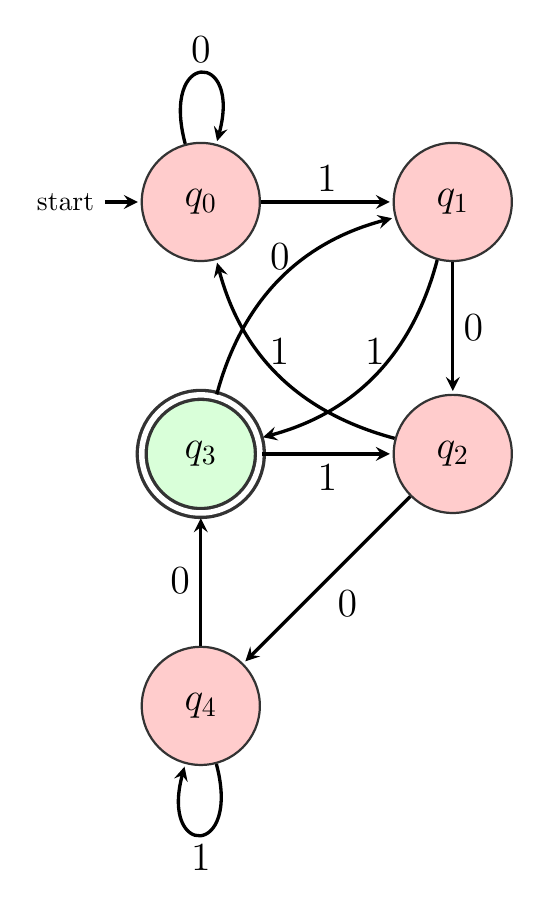
\begin{tikzpicture}[
    shorten >=1pt, 
    node distance=3.2cm, 
    on grid, 
    auto, 
    every state/.style={thick, minimum size=1.5cm, font=\Large, draw=black!80},
    every edge/.append style={line width=1.2pt, >=stealth, shorten >=1pt}
]

   % States
   \node[state, initial, fill=red!20] (q0) {$q_0$}; % initial
   \node[state, fill=red!20] (q1) [right=of q0] {$q_1$};
   \node[state, fill=red!20] (q2) [below=of q1] {$q_2$};
   \node[state, accepting, fill=green!15, double distance=2pt, very thick] (q3) [left=of q2] {$q_3$};
   \node[state, fill=red!20] (q4) [below=of q3] {$q_4$};

   % Transitions (mod 5 machine)
   \path[->]
   (q0) edge [loop above] node {\Large 0} (q0)
        edge node {\Large 1} (q1)

   (q1) edge node {\Large 0} (q2)
        edge[bend left] node [above] {\Large 1} (q3)

   (q2) edge node {\Large 0} (q4)
        edge[bend left] node[above] {\Large 1} (q0)

   (q3) edge[bend left] node[above] {\Large 0} (q1)
        edge node [below] {\Large 1} (q2)

   (q4) edge node[left] {\Large 0} (q3)
        edge[loop below] node[below] {\Large 1} (q4);

\end{tikzpicture}
\section{25 batch}
\subsection{(i) $\varepsilon$-NFA for strings over $\{0,1\}$ with either an even \#0s or an even \#1s}

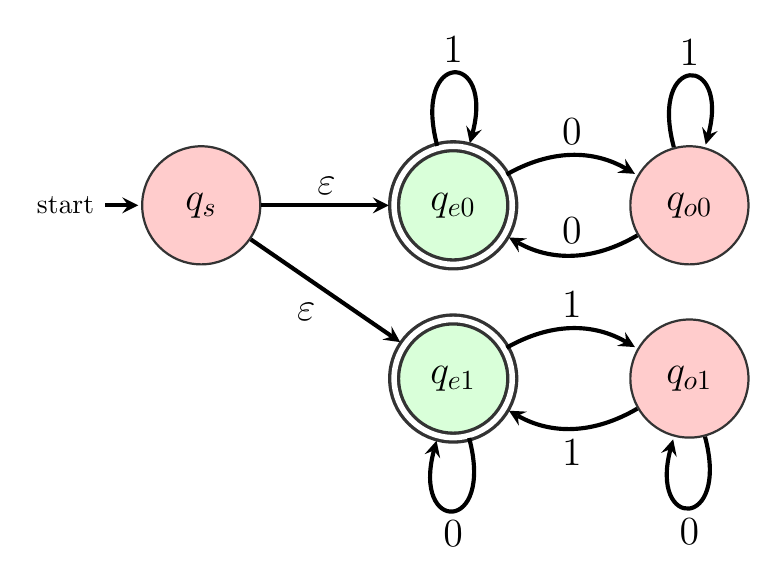
\begin{tikzpicture}[
    shorten >=1pt, 
    node distance=3cm, 
    on grid, 
    auto, 
    every state/.style={thick, minimum size=1.5cm, font=\Large, draw=black!80},
    every edge/.append style={line width=1.5pt, >=stealth, shorten >=1pt}
]

   % States with colors
   \node[state, initial, fill=red!20] (s) {$q_s$};

   % Branch for even number of 0s (ignore 1s)
   \node[state, accepting, fill=green!15, double distance=2pt, very thick] (e0) [right=3.2cm of s] {$q_{e0}$}; % even 0s
   \node[state, fill=red!20] (o0) [right=of e0] {$q_{o0}$}; % odd 0s

   % Branch for even number of 1s (ignore 0s)
   \node[state, accepting, fill=green!15, double distance=2pt, very thick] (e1) [below=2.2cm of e0] {$q_{e1}$}; % even 1s
   \node[state, fill=red!20] (o1) [right=of e1] {$q_{o1}$}; % odd 1s

   % Transitions
   \path[->]
   % epsilon splits
   (s) edge node {\Large $\varepsilon$} (e0)
       edge node[swap] {\Large $\varepsilon$} (e1)

   % Even-0s checker: toggle on 0, ignore 1
   (e0) edge[bend left] node {\Large 0} (o0)
        edge[loop above] node {\Large 1} ()
   (o0) edge[bend left] node [above] {\Large 0} (e0)
        edge[loop above] node {\Large 1} ()

   % Even-1s checker: toggle on 1, ignore 0
   (e1) edge[bend left] node {\Large 1} (o1)
        edge[loop below] node {\Large 0} ()
   (o1) edge[bend left] node {\Large 1} (e1)
        edge[loop below] node {\Large 0} ();
\end{tikzpicture}

\bigskip
\subsection{(ii) Equivalent DFA (subset construction, minimized)}
% States encode parity: (parity of 0s, parity of 1s)
% E = even, O = odd. Accept if either component is even.

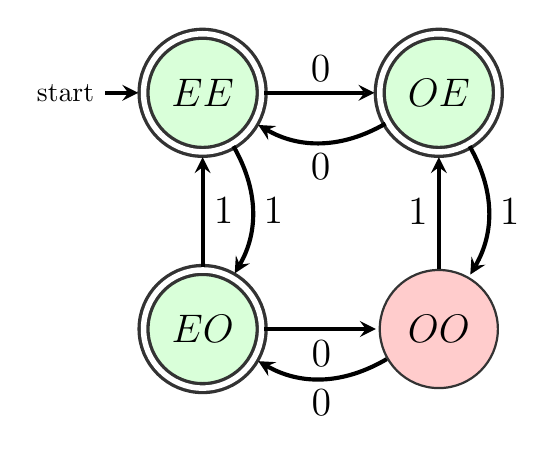
\begin{tikzpicture}[
    shorten >=1pt, 
    node distance=3cm, 
    on grid, 
    auto, 
    every state/.style={thick, minimum size=1.5cm, font=\Large, draw=black!80},
    every edge/.append style={line width=1.5pt, >=stealth, shorten >=1pt}
]

   % States with colors
   \node[state, initial, accepting, fill=green!15, double distance=2pt, very thick] (EE) {$EE$}; % even 0s, even 1s
   \node[state, accepting, fill=green!15, double distance=2pt, very thick] (OE) [right=of EE] {$OE$}; % odd 0s, even 1s
   \node[state, accepting, fill=green!15, double distance=2pt, very thick] (EO) [below=of EE] {$EO$}; % even 0s, odd 1s
   \node[state, fill=red!20] (OO) [right=of EO] {$OO$}; % odd 0s, odd 1s (only reject)

   % Transitions: reading 0 toggles the first component; reading 1 toggles the second
   \path[->]
   (EE) edge node {\Large 0} (OE)
        edge [bend left] node[right] {\Large 1} (EO)

   (OE) edge [bend left] node {\Large 0} (EE)
        edge [bend left] node [right] {\Large 1} (OO)

   (EO) edge node[swap] {\Large 0} (OO)
        edge node[swap] {\Large 1} (EE)

   (OO) edge [bend left] node[below] {\Large 0} (EO)
        edge node {\Large 1} (OE);
\end{tikzpicture}
\section{24 Batch}
\subsection{Three consecutive zeros, not necessarily at the end}
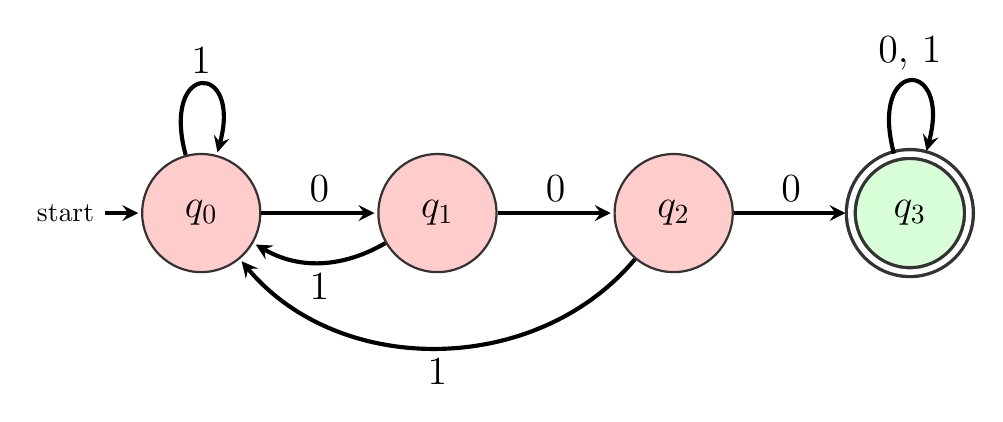
\begin{tikzpicture}[
    shorten >=1pt, 
    node distance=3cm, 
    on grid, 
    auto, 
    every state/.style={thick, minimum size=1.5cm, font=\Large, draw=black!80},
    every edge/.append style={line width=1.5pt, >=stealth, shorten >=1pt}
]

   % States with colors
   \node[state, initial, fill=red!20] (q0) {$q_0$};
   \node[state, fill=red!20] (q1) [right=of q0] {$q_1$};
   \node[state, fill=red!20] (q2) [right=of q1] {$q_2$};
   \node[state, accepting, fill=green!15, double distance=2pt, very thick] (q3) [right=of q2] {$q_3$};

   % Transitions
   \path[->]
   (q0) edge node {\Large 0} (q1)
   (q0) edge [loop above] node {\Large 1} ()

   (q1) edge [bend left] node {\Large 1} (q0)
   (q1) edge node {\Large 0} (q2)
   (q2) edge [bend left = 50] node {\Large 1} (q0)
   (q3) edge [loop above] node {\Large 0, 1} ()
   (q2) edge node {\Large 0} (q3); % loop for both 'a' and 'b'
\end{tikzpicture}
\[
\Huge \mathbf{
(0+1)^{*} \, 000 \, (0+1)^{*}
}
\]

\section{23 Batch}
\subsection{Ends with 01}
\paragraph{NFA}
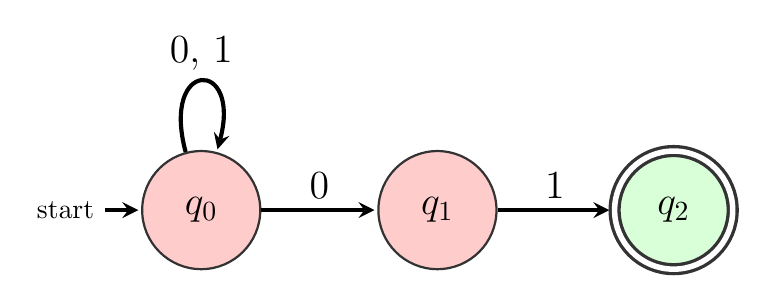
\begin{tikzpicture}[
    shorten >=1pt, 
    node distance=3cm, 
    on grid, 
    auto, 
    every state/.style={thick, minimum size=1.5cm, font=\Large, draw=black!80},
    every edge/.append style={line width=1.5pt, >=stealth, shorten >=1pt}
]

   % States with colors
   \node[state, initial, fill=red!20] (q0) {$q_0$};
   \node[state, fill=red!20] (q1) [right=of q0] {$q_1$};
   \node[state, accepting, fill=green!15, double distance=2pt, very thick] (q2) [right=of q1] {$q_2$};

   % Transitions
   \path[->]
   (q0) edge node {\Large 0} (q1)
   (q0) edge [loop above] node {\Large 0, 1} ()

   (q1) edge node {\Large 1} (q2);
\end{tikzpicture}

\paragraph{DFA}
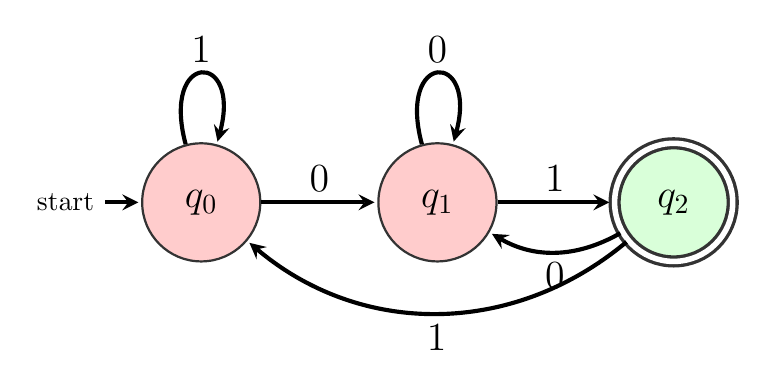
\begin{tikzpicture}[
    shorten >=1pt, 
    node distance=3cm, 
    on grid, 
    auto, 
    every state/.style={thick, minimum size=1.5cm, font=\Large, draw=black!80},
    every edge/.append style={line width=1.5pt, >=stealth, shorten >=1pt}
]

   % States with colors
   \node[state, initial, fill=red!20] (q0) {$q_0$};
   \node[state, fill=red!20] (q1) [right=of q0] {$q_1$};
   \node[state, accepting, fill=green!15, double distance=2pt, very thick] (q2) [right=of q1] {$q_2$};

   % Transitions
   \path[->]
   (q0) edge node {\Large 0} (q1)
   (q0) edge [loop above] node {\Large  1} ()
   (q1) edge [loop above] node {\Large  0} ()
   (q2) edge [bend left = 40] node {\Large 1} (q0)
   (q2) edge [bend left] node {\Large 0} (q1)

   (q1) edge node {\Large 1} (q2);
\end{tikzpicture}
\subsection{Even number of 1 and even number of 0}
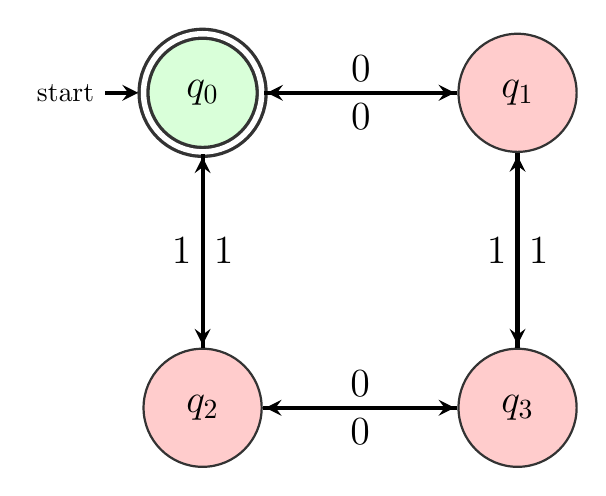
\begin{tikzpicture}[
    shorten >=1pt, 
    node distance=4cm, 
    on grid, 
    auto, 
    every state/.style={thick, minimum size=1.5cm, font=\Large, draw=black!80},
    every edge/.append style={line width=1.5pt, >=stealth, shorten >=1pt}
]

   % States
   \node[state, initial, accepting, fill=green!15, double distance=2pt, very thick] (q0) {$q_0$}; % even 0s, even 1s
   \node[state, fill=red!20] (q1) [right=of q0] {$q_1$}; % odd 0s, even 1s
   \node[state, fill=red!20] (q2) [below=of q0] {$q_2$}; % even 0s, odd 1s
   \node[state, fill=red!20] (q3) [right=of q2] {$q_3$}; % odd 0s, odd 1s

   % Transitions
   \path[->]
   (q0) edge node {\Large 0} (q1)
        edge node[swap] {\Large 1} (q2)

   (q1) edge node {\Large 0} (q0)
        edge node {\Large 1} (q3)

   (q2) edge node[swap] {\Large 0} (q3)
        edge node[swap] {\Large 1} (q0)

   (q3) edge node[swap] {\Large 0} (q2)
        edge node {\Large 1} (q1);
\end{tikzpicture}

\subsection{Odd number of 1}
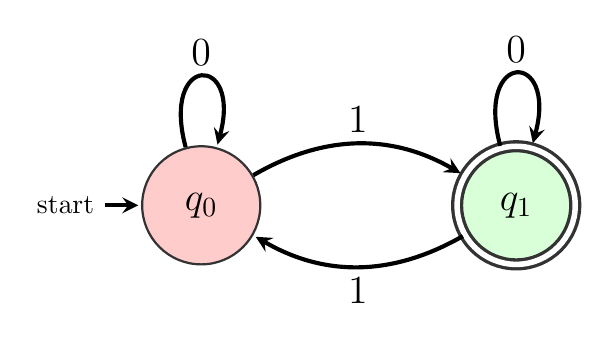
\begin{tikzpicture}[
    shorten >=1pt, 
    node distance=4cm, 
    on grid, 
    auto, 
    every state/.style={thick, minimum size=1.5cm, font=\Large, draw=black!80},
    every edge/.append style={line width=1.5pt, >=stealth, shorten >=1pt}
]

   % States
   \node[state, initial, fill=red!20] (q0) {$q_0$}; % even # of 1s
   \node[state, accepting, fill=green!15, double distance=2pt, very thick] (q1) [right=of q0] {$q_1$}; % odd # of 1s

   % Transitions
   \path[->]
   (q0) edge[loop above] node {\Large 0} ()
        edge[bend left] node {\Large 1} (q1)

   (q1) edge[loop above] node {\Large 0} ()
        edge[bend left] node {\Large 1} (q0);
\end{tikzpicture}
\section{Even number of a and odd number of b and not containing substring ab}
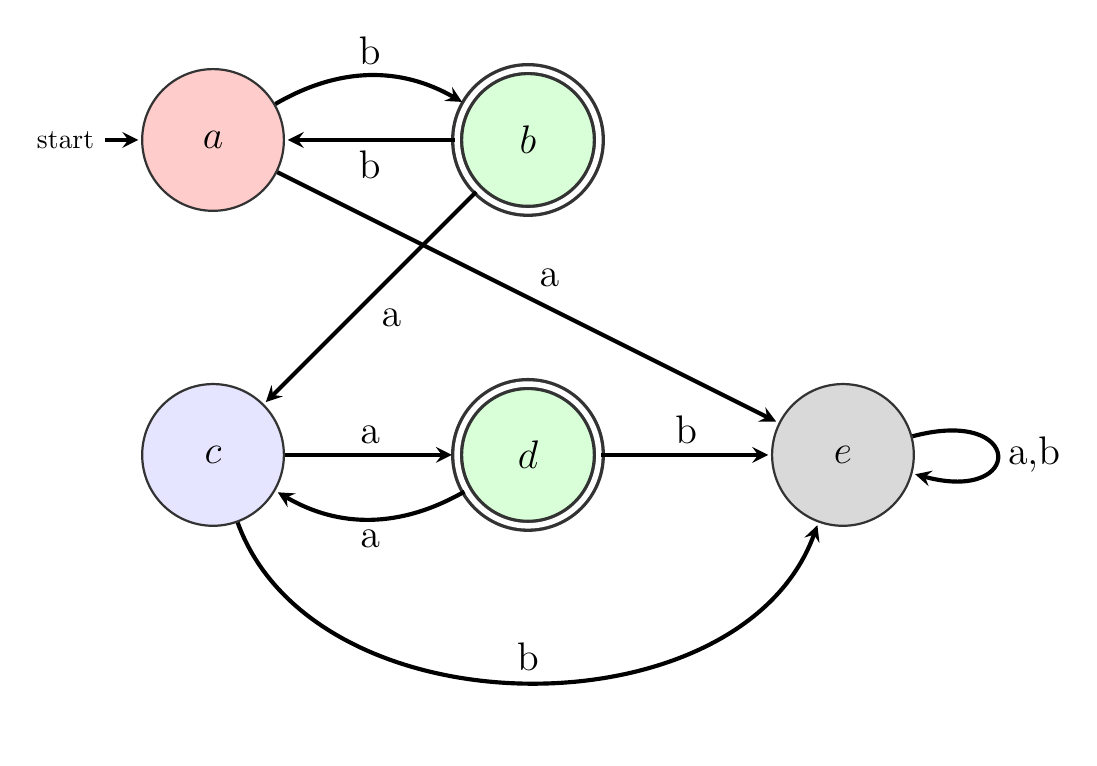
\begin{tikzpicture}[
    shorten >=1pt, 
    node distance=4cm, 
    on grid, 
    auto, 
    every state/.style={thick, minimum size=1.8cm, font=\Large, draw=black!80},
    every edge/.append style={line width=1.5pt, >=stealth, shorten >=1pt}
]

   % States
   \node[state, initial, fill=red!20]                        (a) {$a$}; % start: before any a, b-parity even (reject)
   \node[state, accepting, fill=green!15, double distance=2pt, very thick] (b) [right=of a] {$b$}; % before any a, b-parity odd (accept)

   \node[state, fill=blue!10]  (c) [below=of a] {$c$}; % after first a: b-parity odd, a-parity odd (reject)
   \node[state, accepting, fill=green!15, double distance=2pt, very thick] (d) [right=of c] {$d$}; % after a: b-parity odd, a-parity even (accept)

   \node[state, fill=gray!30] (e) [right=of d] {$e$}; % sink: unrecoverable rejects

   % Transitions in b*-phase
   \path[->]
     (a) edge[bend left] node {\Large b} (b)
     (b) edge node {\Large b} (a);

   % Transitions from b*-phase to a*-phase
   \path[->]
     (a) edge node {\Large a} (e)   % entering a-phase with b even -> sink (unrecoverable)
     (b) edge node {\Large a} (c);  % entering a-phase with b odd -> a-parity odd (c)

   % a-phase toggling on 'a'
   \path[->]
     (c) edge node {\Large a} (d)
     (d) edge[bend left] node {\Large a} (c);

   % b after entering a-phase -> sink
   \path[->]
     (c) edge [bend right = 70 ] node {\Large b} (e)
     (d) edge node {\Large b} (e);

   % sink state loop
   \path[->]
     (e) edge[loop right] node {\Large a,b} ();

\end{tikzpicture}
\[
\Huge \mathbf{
b (bb)^{*} (aa)^{*}
}
\]

\section{\[
L = \{\, w \mid w \text{ has an odd number of } a\text{'s and ends with a } b \,\}
\]
}
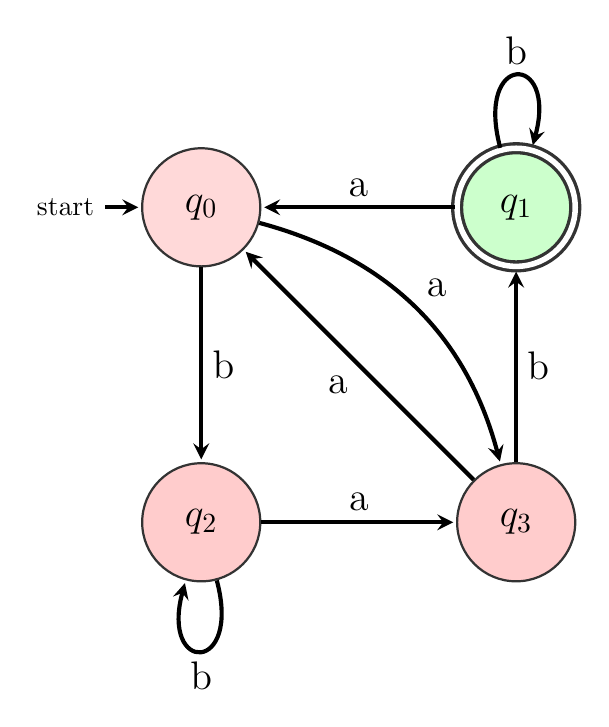
\begin{tikzpicture}[
    shorten >=1pt, 
    node distance=4cm, 
    on grid, 
    auto, 
    every state/.style={thick, minimum size=1.5cm, font=\Large, draw=black!80},
    every edge/.append style={line width=1.5pt, >=stealth, shorten >=1pt}
]

   % States
   \node[state, initial, fill=red!15] (q0) {$q_0$}; % even 0s, even 1s
   \node[state, fill=green!20,accepting, double distance=2pt, very thick] (q1) [right=of q0] {$q_1$}; % odd 0s, even 1s
   \node[state, fill=red!20] (q2) [below=of q0] {$q_2$}; % even 0s, odd 1s
   \node[state, fill=red!20] (q3) [right=of q2] {$q_3$}; % odd 0s, odd 1s

   % Transitions
   \path[->]
   (q0) edge node {\Large b} (q2)
        edge [bend left] node {\Large a} (q3)
   (q1) edge node [above] {\Large a} (q0)
        edge [loop above] node {\Large b} (q3)

   (q2) edge node {\Large a} (q3)
        edge [loop below] node {\Large b} ()

   (q3) edge node [right] {\Large b} (q1)
        edge node {\Large a} (q0);
\end{tikzpicture}
\section{Has even length and an odd number of a’s}
\begin{center}
    \includegraphics[width=1.3\textwidth]{extra/1.png}
\end{center}
\section{Qs}
\begin{center}
    \includegraphics[width=1.3\textwidth]{extra/2.png} % replace logo.png with your file
\end{center}
\section{Qs}
\begin{center}
    \includegraphics[width=1.3\textwidth]{extra/3.png} % replace logo.png with your file
\end{center}



\end{document}

